\documentclass{article}

\usepackage{titlesec}
\newcommand{\sectionbreak}{\clearpage}

\usepackage{fancyhdr}
\pagestyle{fancy}
\lhead{Emanuel Casiano-Diaz}
\rhead{CSYS300: PoCS - Homework 01 - 09/07/2018}
\renewcommand{\headrulewidth}{0.4pt}
\renewcommand{\footrulewidth}{0.4pt}

\usepackage{amsmath}
\usepackage{amssymb}
\usepackage{bm}
\usepackage{pdfpages}

\usepackage{enumerate}% http://ctan.org/pkg/enumerate

\usepackage{hyperref}
\hypersetup{
    colorlinks=true,
    linkcolor=blue,
    filecolor=magenta,      
    urlcolor=cyan,
}


\begin{document}

\section{Exercise 1}

Code used throughout the assignment can be found in the following git repository: \url{https://github.com/ecasiano/PrinciplesOfComplexSystems}


\begin{figure}[h!]
  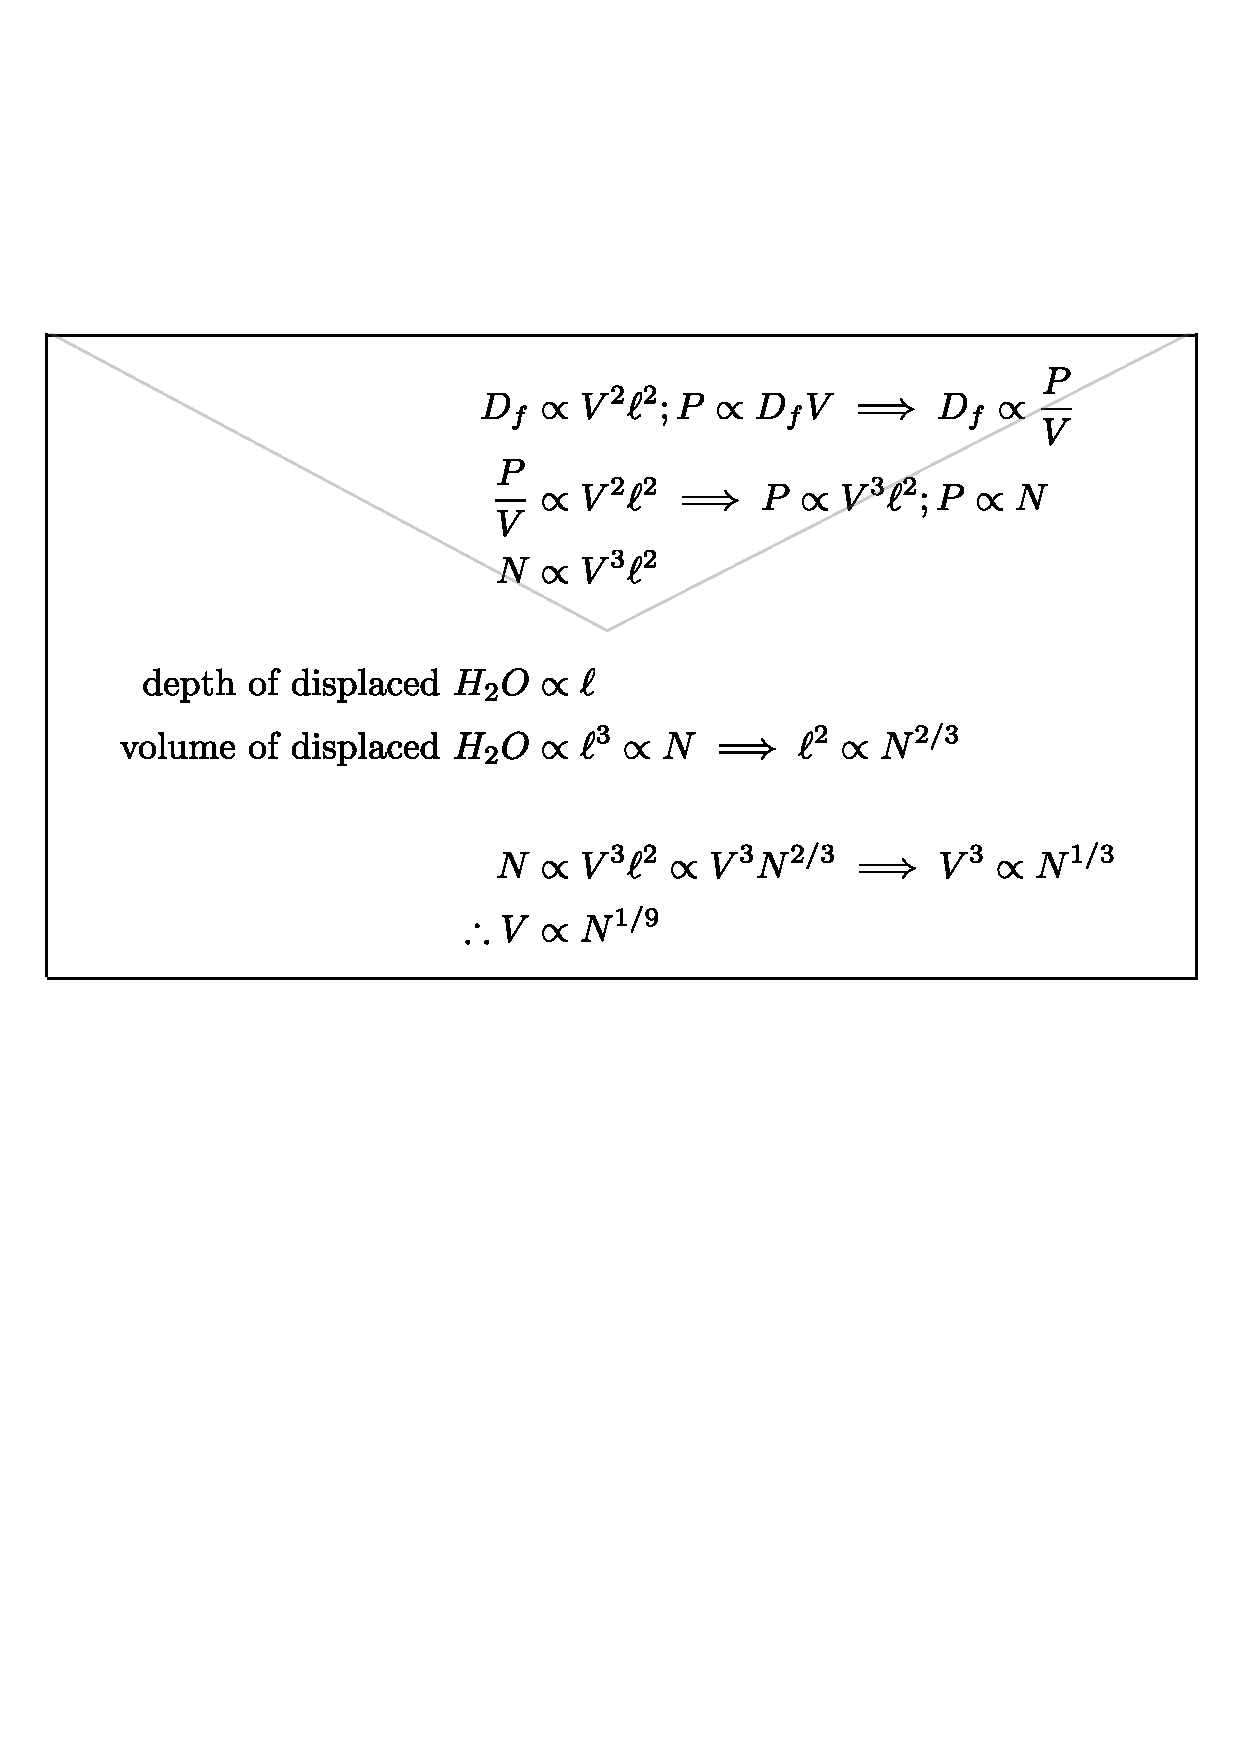
\includegraphics[width=\linewidth]{Q01/powerLawEnvelope.pdf}
  \caption{The above figure shows the back of the actual envelope on which the power law scaling of shell velocity, $V$, as a function of total oarspeople, $N$, was derived.}
  \label{fig:envelope}
\end{figure}

\section{Exercise 2}

Current rowing best times can be found here:\url{https://en.wikipedia.org/wiki/List_of_world_records_in_rowing}

\begin{figure}[h!]
  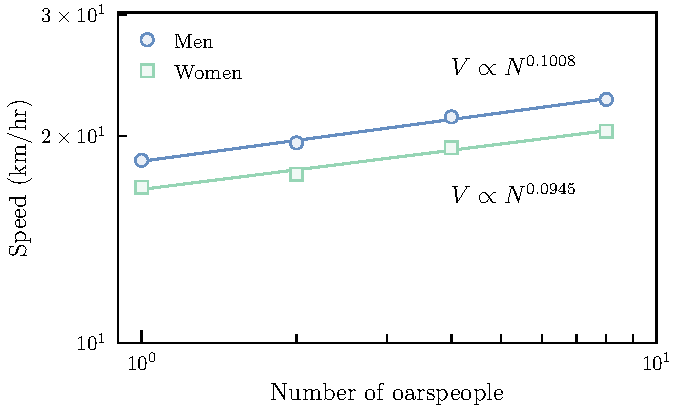
\includegraphics[width=\linewidth]{Q02/rowingPowerLaw.pdf}
  \caption{Speed of shell,V, as a function of number of oarspeople, N}
  \label{fig:rowingPowerLawPlot}
\end{figure}

As per the current best times in rowing, McMahon and Bonner's power law of $S \propto N^{1/9}$ still holds. Since $1/9 = 0.\overline{1111}$, the relative error with respect to the men data is $\approx 9.28\%$, which is not too bad considering the very small number of data points. With the small number of data points, variations in the values of speeds should affect the scaling more than if many points were plotted, yet the relative error is only $9.28\%$

\section{Exercise 3}

Current weightlifting records can be found here: \url{https://en.wikipedia.org/wiki/List_of_world_records_in_Olympic_weightlifting}

\begin{figure}[h]
  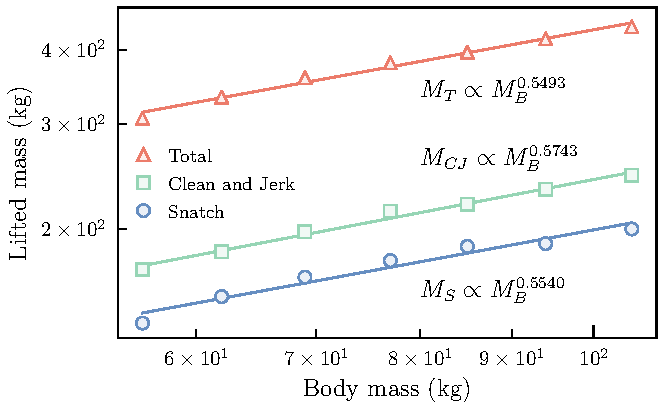
\includegraphics[width=\linewidth]{Q03/liftingPowerLaw.pdf}
  \caption{Lifted mass as a function of body mass of the lifter. Results have been plotted for three weightlifting events: Snatch, Clean \& Jerk and Total. Annotations next to each curve describe their power law scaling.}
  \label{fig:liftingPowerLawPlot}
\end{figure}
\begin{figure}[t]
  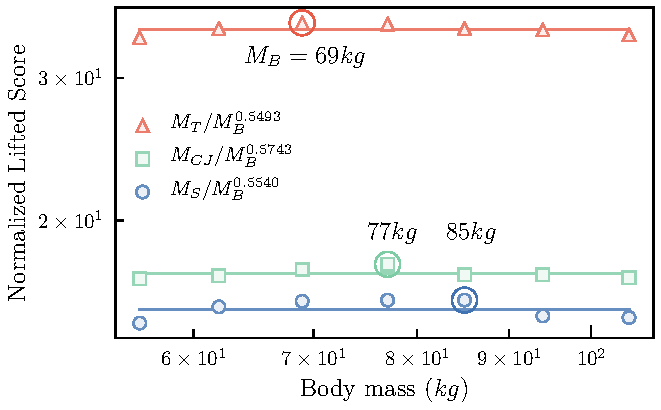
\includegraphics[width=\linewidth]{Q03/liftingPowerLawNormed.pdf}
  \caption{Normalized lifted "score", $M_{Event}*M_B^{-x}$, where $x$ is the scaling exponent, as a function of body mass. The circled data points correspond to the "strongest" lifter of each event.}
  \label{fig:liftingPowerLawPlot}
\end{figure}

\section{Exercise 4}

Parameters and their dimensions: \begin{align}
[\ell] &= L \\
[m] &= M \\
[g] &= LT^{-2} \\
[\tau] &= T
\end{align}

where $L,M$ and $T$ are units if length, mass and time, respectively.

Via the Buckingham-$Pi$ Theorem:

\begin{equation}
[\pi_1] = L^{x_1} M^{x_2} L^{x_3} T^{-2x_3} T^{x_4} = L^{(x_1 + x_3)} M^{x_2} T^{(-2x_3 + x_4)}   = 1
\end{equation}

the exponents of each dimension should be each equal to zero. Thus, a system of 3 linear equations in 4 unknowns is obtained, which can be solved with Matrixology:

\begin{equation}
A\bm{x} = \begin{pmatrix}
1&0&1&0 \\
0&1&0&0 \\
0&0&-2&1 \\
\end{pmatrix}
\begin{pmatrix}
x_1\\
x_2\\
x_3\\
x_4\\
\end{pmatrix}
=
\begin{pmatrix}
0\\
0\\
0\\
\end{pmatrix}
\end{equation}

which can be rewritten in Reduced Row Echelon form by applying Elementary Row Operations as:

\begin{equation}
A\bm{x} = \begin{pmatrix}
1&0&1&0 \\
0&1&0&0 \\
0&0&1&-\frac{1}{2} \\
\end{pmatrix}
\begin{pmatrix}
x_1\\
x_2\\
x_3\\
x_4\\
\end{pmatrix}
=
\begin{pmatrix}
0\\
0\\
0\\
\end{pmatrix}
\end{equation}

to give the three equations:

\begin{align}
x_1 + x_3 &= 0 \\
x_2 &= 0 \\
x_3 - \frac{1}{2} x_4 &= 0 
\end{align}

with solution:

\begin{equation}
\begin{pmatrix}
x_1\\
x_2\\
x_3\\
x_4\\
\end{pmatrix}
= x_3
\begin{pmatrix}
-1\\
0\\
1\\
2\\
\end{pmatrix}
\end{equation}

Then, substituting into the $pi_1$ group:

\begin{equation}
\pi_1 = \ell^{x_1} m^{x_2} g^{x_3} \tau^{x_4} = \ell g^{-1} \tau{-2} = \text{ const.} \implies \tau \propto \sqrt{\ell/g} 
\end{equation}

\section{Exercise 5}

Parameters and their dimensions: \begin{align}
[V_{max}] &= LT^{-1}\\
[\ell] &= L \\
[\rho] &= ML^{-3} \\
[\sigma] &= ML^{-1}T^{-2} \\
[b] &= L^2T^{-3}
\end{align}

Define $V_{max}/\ell \equiv \bar{V}$ such that $[\bar{V}] = T^{-1}$ \\

Want to show that $V_{max} \propto \ell$, given that $b\rho/\sigma \approx \text{ const.}$ \\

Check: 

From the $\sigma$ equation:
\begin{align}
\sigma &\propto ML^{-1}T^{-2} \\
\implies \sigma M^{-1} L &\propto T^{-2}\\
\implies \sigma M^{-1} L T^{-1} &\propto T^{-3} 
\end{align}

From the b equation:
\begin{align}
b &\propto L^2 T^{-3} \\
\implies bL^{-2} &\propto T^{-3} \\
bL^{-2} &\propto  (\sigma M^{-1} L T^{-1}) \\
\implies b &\propto \sigma M^{-1} L^3 T^{-1} 
\end{align}

"Solving" for $T^{-1}$:
\begin{align}
T^{-1} &\propto b \sigma^{-1} ML^{-3} ; ML^{-3} \text{ are units of volume!} \\
T^{-1} &\propto b \sigma^{-1} \rho ; T^{-1} \text{ are units of speed over length!} \\
\implies \bar{V} = V_{max}/\ell &\propto b \rho / \sigma \approx \text{ const.}
\end{align}

\[ \therefore V_{max} \propto \ell \]

\section{Exercise 6}

Parameters and their dimensions: \begin{align}
[E] &= ML^2T^{-2} \\
[\rho] &= ML^{-3} \\
[R] &= L \\
[t] &= T
\end{align}

Via the Buckingham-$\pi$ Theorem:
\[ [\pi_1] = [E]^{x_1}[\rho]^{x_2}[R]^{x_3}[t]^{x_4} = M^{(x_1+x_2)}L^{(2x_1-3x_2+x_3)}T^{(-2x_1+x_4)} = 1\]

This time, the $A\bm{x}=\bm{0}$ problem we need to solve becomes:

\begin{equation}
A\bm{x} = \begin{pmatrix}
1&1&0&0 \\
2&-3&1&0 \\
-2&0&0&1 \\
\end{pmatrix}
\begin{pmatrix}
x_1\\
x_2\\
x_3\\
x_4\\
\end{pmatrix}
=
\begin{pmatrix}
0\\
0\\
0\\
\end{pmatrix}
\end{equation}

which can be rewritten in Reduced Row Echelon form by applying Elementary Row Operations as:

\begin{equation}
A\bm{x} = \begin{pmatrix}
1&1&0&0 \\
0&1&-\frac{1}{5}&0 \\
0&0&1&\frac{5}{2} \\
\end{pmatrix}
\begin{pmatrix}
x_1\\
x_2\\
x_3\\
x_4\\
\end{pmatrix}
=
\begin{pmatrix}
0\\
0\\
0\\
\end{pmatrix}
\end{equation}

to give the three equations:

\begin{align}
x_1 + x_2 &= 0 \\
x_2 - \frac{1}{5} x_3 &= 0 \\
x_3 + \frac{5}{2} x_4 &= 0 
\end{align}

with solution:

\begin{equation}
\begin{pmatrix}
x_1\\
x_2\\
x_3\\
x_4\\
\end{pmatrix}
= x_4
\begin{pmatrix}
1/2\\
-1/2\\
-5/2\\
1\\
\end{pmatrix}
\end{equation}

Then, substituting into the $pi_1$ group:

\begin{equation}
\pi_1 = E^{1/2}\rho^{-1/2}R^{-5/2} = \text{ const.} \implies E \propto \rho R^5 /t^2
\end{equation}

\section{Exercise 7}

Parameters and their dimensions: \begin{align}
[m_E] &= [m_S] = M \\
[\tau] &= T \\
[r] &= L \\
[G] &= L^3 M^{-1} T^{-2}
\end{align}

Via the Buckingham-$\pi$ Theorem:
\[ [\pi_1] = [m_E]^{x_1}[\tau]^{x_2}[r]^{x_3}[G]^{x_4} = M^{(x_1-x_4)}T^{(x_2-2x_4)}L^{(x_3+3x_4)} = 1\]

This time, the $A\bm{x}=\bm{0}$ problem we need to solve becomes:

\begin{equation}
A\bm{x} = \begin{pmatrix}
1&0&0&-1 \\
0&1&0&-2 \\
0&0&1&3 \\
\end{pmatrix}
\begin{pmatrix}
x_1\\
x_2\\
x_3\\
x_4\\
\end{pmatrix}
=
\begin{pmatrix}
0\\
0\\
0\\
\end{pmatrix}
\end{equation}

which is already in Reduced Row Echelon form and gives the three equations:

to give the three equations:

\begin{align}
x_1 - x_4 &= 0 \\
x_2 - 2 x_4 &= 0 \\
x_3 + 3 x_4 &= 0 
\end{align}

with solution:

\begin{equation}
\begin{pmatrix}
x_1\\
x_2\\
x_3\\
x_4\\
\end{pmatrix}
= x_4
\begin{pmatrix}
1\\
2\\
-3\\
1\\
\end{pmatrix}
\end{equation}

Then, substituting into the $\pi_1$ group:

\[ \pi_1 = m_E\tau^{2}r^{-3}G =  \text{ const.} \implies \tau^2 \propto r^3 \]


\begin{figure}[h!]
  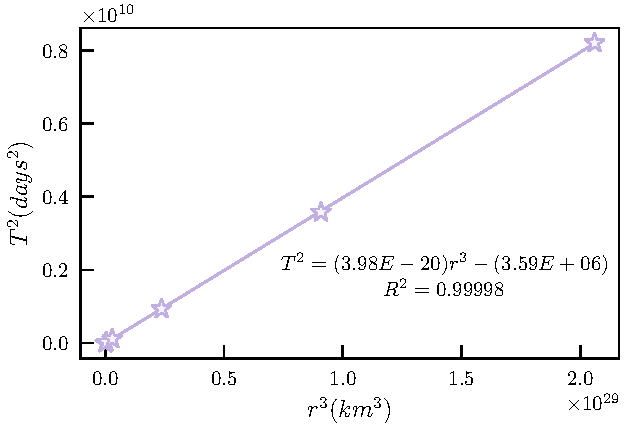
\includegraphics[width=\linewidth]{Q07/keplerLawPlot.pdf}
  \caption{Square of the orbital period as a function of the cube of the orbital radii for each planet in the Solar System, including Pluto. From Kepler's Law, it is expected that the plot should be a line. After doing a linear regression, the coefficient of determination obtained, $R^2 \approx 1$ confirms that Kepler's Law holds in the Solar System. Data can be found at: \url{https://nssdc.gsfc.nasa.gov/planetary/factsheet/}} 
  \label{fig:keplerLawPlot}
\end{figure}

\section{Exercise 8}

\subsection{}

\[ L_i = c_i^{-1}V^{\gamma_i}\]

where $i={1,2,3}$, $\sum_i \gamma_i = 1$ and $\Pi_i c_i = 1$.

\[ L_1 L_2 L_3 = (c_1c_2c_3)^{-1} V ^{\gamma_1 + \gamma_2 + \gamma_3} = V\] \\

\subsection{}

The isometric scaling exponent in this system is: $\gamma_i = 1/3$ for $i={1,2,3}$ \\

\subsection{}

The surface area, $S$, is the total of the area of each face of the Minecraft organisms. Thus:

\begin{align}
S(V) &= 2L_1L_2 + 2L_2L_3 + 2L_3L_1 \\
S &= 2[(c_1c_2)^{-1} V^{\gamma_1 + \gamma_2} + (c_2c_3)^{-1} V^{\gamma_2 + \gamma_3} + (c_3c_1)^{-1} V^{\gamma_3 + \gamma_1}] \\
S(V) &= 2[c_3V^{\gamma_1 + \gamma_2} + c_1 V^{\gamma_2 + \gamma_3} + c_2 V^{\gamma_3 + \gamma_1}]
\end{align}

\subsection{}

Since $\gamma_1 \leq \gamma_2 \leq \gamma_3$, the second term in the above expression has the largest exponent. Thus, for large $V$, this term will dominate and the surface area will goes as:

\[ S(V) \approx 2c_1 V^{(\gamma_2+\gamma_3)}\]

\subsection{}

Fastest scaling of $S(V)$: $\gamma_1 = 0, \gamma_2 = 0, \gamma_3 = 1$ \\
Slowest scaling of $S(V)$: $\gamma_1 = 1/3, \gamma_2 = 1/3, \gamma_3 = 1/3$ (Isometric Scaling) \\

NOTE: The figure in the next page confirms these predictions.


\begin{figure}[h!]
  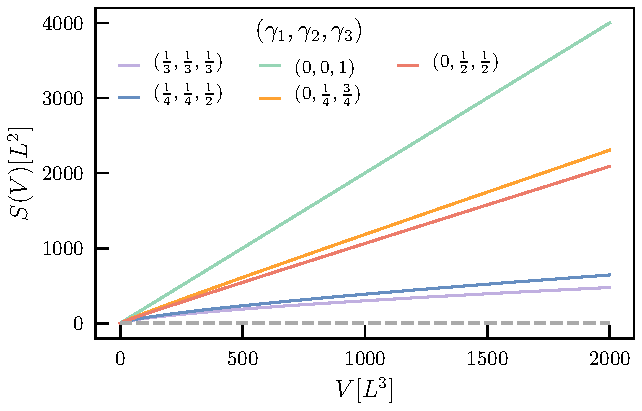
\includegraphics[width=\linewidth]{Q08/minecraftConvergence.pdf}
  \caption{Surface area as a function of volume. Different sets of $\gamma_i$ have been chosen to test the predictions for the scaling of $S$. For plotting purposes $2c_i$ has been set to $1$ for $i={1,2,3}$. }
  \label{fig:minecraftConvergence}
\end{figure}

\end{document}